% ===============================
%          Chapter 1B.2
%     The Roles of the Blood
%     Created by Michael Tang
%           2025.01.01
% ===============================

\subsubsection{1B.2 The Roles of the Blood}
\paragraph{The \underline{Cardiovascular System} (心血管系统)}
\begin{itemize}
    \item The cardiovascular system is a mass transport system in mammals, consisting of:
    \begin{itemize}
        \item[1.] \textbf{Heart:} Pumps blood.
        \item[2.] \textbf{Blood vessels:} Transport blood to tissues.
        \item[3.] \textbf{Blood:} The transport medium carrying nutrients, gases, hormones, and waste.
    \end{itemize}
    \item Functions:
    \begin{itemize}
        \item Delivers materials like oxygen and glucose to body cells.
        \item Removes waste products (e.g., carbon dioxide, urea).
        \item Distributes heat and maintains body temperature.
    \end{itemize}
\end{itemize}

\paragraph{Components of Blood}
\begin{figure}[H]
    \centering
    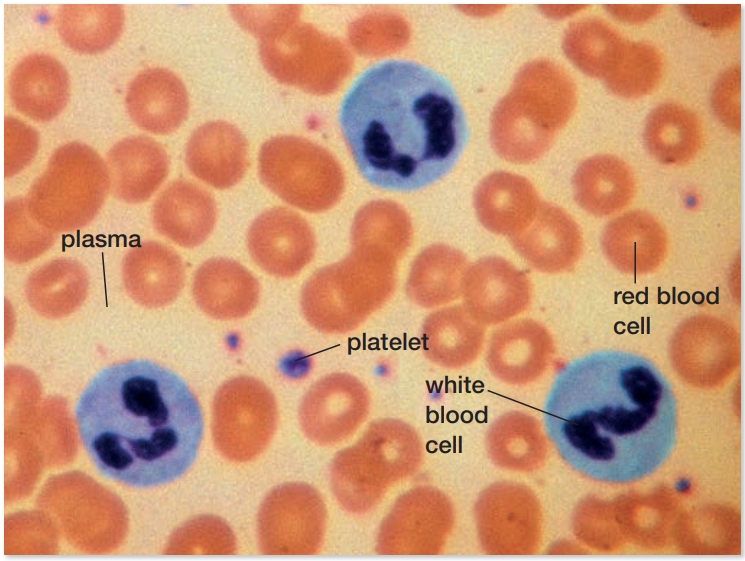
\includegraphics[scale=0.25]{Biology/1B/Images/1B-2-1.png}
    \caption{This light micrograph shows red blood cells, white blood cells and platelets.}
\end{figure}
\begin{itemize}
    \item[1.] \textbf{\underline{Plasma} (血浆):}
    \begin{itemize}
        \item Liquid part of blood ($55\%$ of blood volume).
        \item Transport:
        \begin{itemize}
            \item Digested food (e.g., glucose, amino acids).
            \item \underline{Excretory products} (排泄物 e.g., urea, carbon dioxide).
            \item Hormones.
        \end{itemize}
        \item Maintains a stable pH and regulates body temperature.
    \end{itemize}
    \item[2.] \textbf{\underline{Erythrocytes} (红细胞 Red Blood Cells):}
    \begin{itemize}
        \item Approximately 4-6 million cells per $\text{mm}^3$.
        \item Contain haemoglobin to transport oxygen.
        \item Adaptations:
        \begin{itemize}
            \item \underline{Biconcave} (双凹面) shape increases surface area.
            \item No nucleus allows more haemoglobin storage.
            \item \underline{Lifespan} (寿命) of $\sim 120$ days.
        \end{itemize}
    \end{itemize}
    \item[3.] \textbf{\underline{Leukocytes} (白细胞 White Blood Cells):}
    \begin{itemize}
        \item Approximately 4,000-11,000 cells per $\text{mm}^3$.
        \item Role:
        \begin{itemize}
            \item Defend against \underline{pathogens} (病原体 e.g., bacteria, viruses).
            \item Aid in \underline{inflammatory response} (炎症反应).
        \end{itemize}
        \item Types:
        \begin{itemize}
            \item \underline{Granulocytes} (contain granules 粒细胞 e.g., neutrophils 嗜中性粒细胞, eosinophils 嗜酸性粒细胞).
            \item \underline{Agranulocytes} (no granules 无颗粒细胞 e.g., lymphocytes 淋巴细胞, monocytes 单核细胞).
        \end{itemize}
    \end{itemize}
    \item[4.] \textbf{\underline{Platelets} (血小板):}
    \begin{itemize}
        \item Small cell \underline{fragments} (片段) without a nucleus ($\sim 150,000-400,000$ per $\text{mm}^3$).
        \item Involved in \underline{blood clotting} (凝血).
    \end{itemize}
\end{itemize}

\paragraph{Transport of Oxygen}
\begin{itemize}
    \item Haemoglobin binds oxygen in the lungs and forms \underline{oxyhaemoglobin} (氧合血红蛋白):
    \begin{equation}
        \frac{\ce{Hb + 4O2 <=> Hb.4O2}}{\ce{Haemoglobin + Oxygen <=> Oxyhaemoglobin}}
    \end{equation}
    \item Oxygen \underline{dissociation curve} (氧解离曲线):
    \begin{itemize}
        \item S-shaped curve showing \underline{haemoglobin saturation} (血红蛋白饱和度) at different oxygen pressures.
        \item In low oxygen environments, haemoglobin releases oxygen to tissues efficiently.
    \end{itemize}
    \begin{figure}[H]
        \centering
        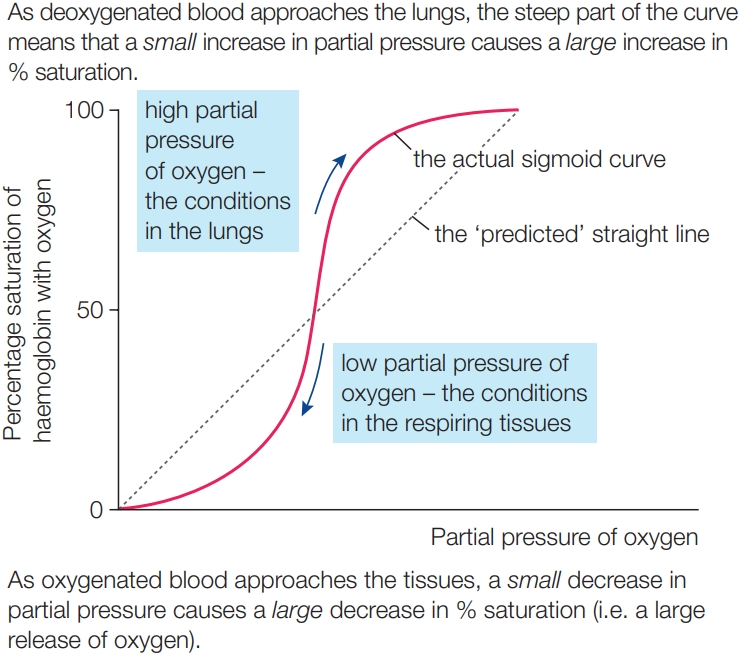
\includegraphics[scale=0.25]{Biology/1B/Images/1B-2-2.png}
        \caption{Oxygen dissociation curve for human haemoglobin.}
    \end{figure}
\end{itemize}

\paragraph{Transport of Carbon Dioxide}
\begin{itemize}
    \item Carbon dioxide is transported in three forms:
    \begin{itemize}
        \item[1.] Dissolved in plasma ($5\%$).
        \item[2.] Bound to haemoglobin as carbaminohaemoglobin ($10-20\%$).
        \item[3.] As \underline{bicarbonate ions} ($\ce{HCO3-}$ 碳酸氢根离子) in plasma ($70-85\%$, majority).
    \end{itemize}
    \item The reaction of the carbon dioxide with water is crucial. When carbon dioxide is dissolved in the blood it reacts
    slowly with the water to form carbonic acid (\ce{H2CO3}). The carbonic acid separates to form hydrogen ions (\ce{H+}) and
    hydrogencarbonate ions (\ce{HCO3-}):
    \begin{equation}
        \ce{CO2 + H2O <=> H2CO3 <=> H+ + HCO3-}
    \end{equation}
    \item \textbf{\underline{Chloride shift} (氯离子转移):} Exchange of bicarbonate ions for chloride ions in red blood cells
    maintains charge balance.
    \begin{figure}[H]
        \centering
        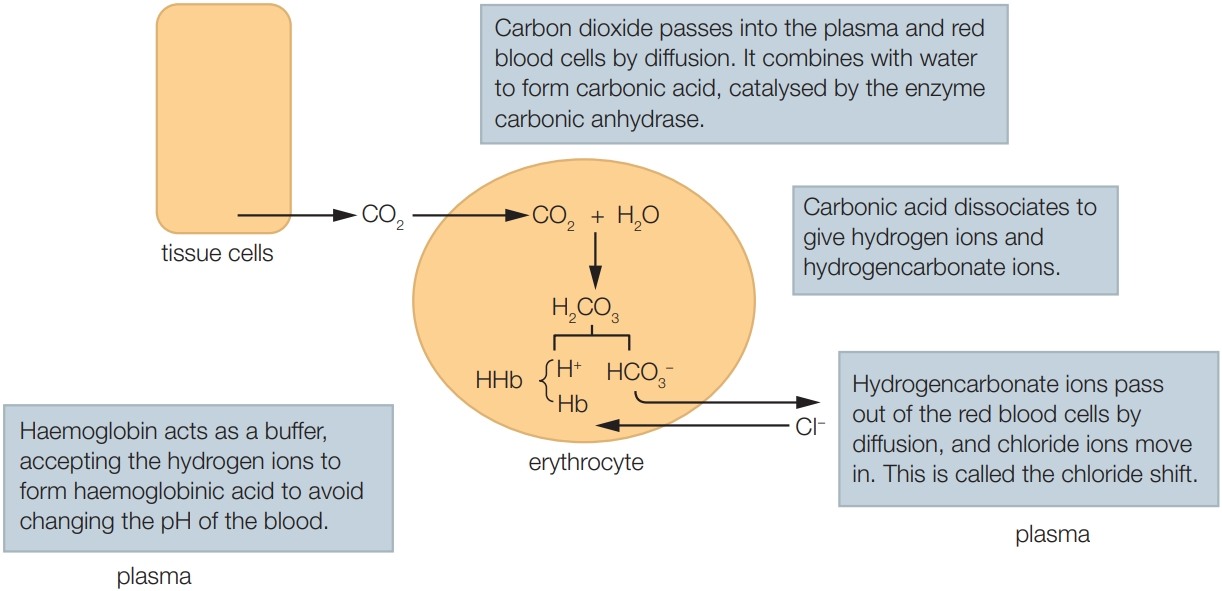
\includegraphics[scale=0.25]{Biology/1B/Images/1B-2-3.png}
        \caption{The transport of carbon dioxide from the tissues to the lungs depends on the reaction of carbon dioxide with
        water, controlled by an enzyme in the red blood cells.}
    \end{figure}
\end{itemize}

\paragraph{\underline{The Bohr Effect} (波尔效应)}
High carbon dioxide levels in active tissues lower haemoglobin's affinity for oxygen, allowing oxygen to be released more readily.
The changes in the oxygen dissociation curve that result as the carbon dioxide level changes are known as the Bohr effect.
\begin{figure}[H]
    \centering
    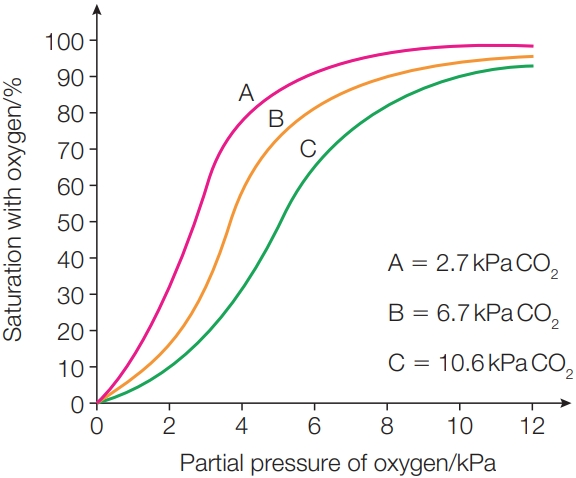
\includegraphics[scale=0.25]{Biology/1B/Images/1B-2-4.png}
    \caption{As the proportion of carbon dioxide in the environment rises, the haemoglobin curve moves down and to the right, so
    it gives up oxygen more easily. This is known as the Bohr effect.}
\end{figure}

\paragraph{\underline{Fetal Haemoglobin} (胎儿血红蛋白)}
Fetal haemoglobin has a higher oxygen affinity than adult haemoglobin, enabling oxygen transfer from the mother's blood to the
fetus.
\begin{figure}[H]
    \centering
    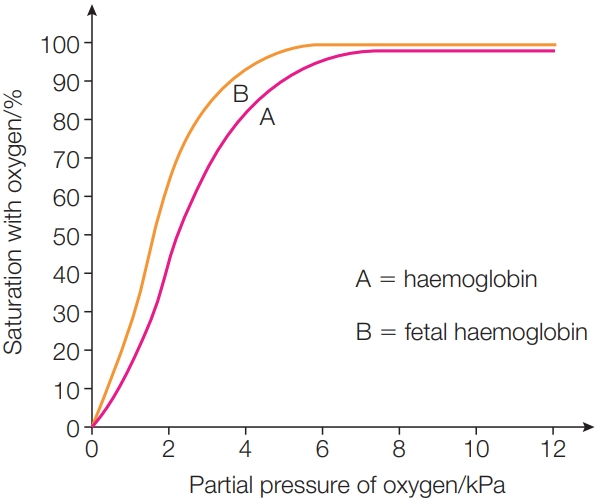
\includegraphics[scale=0.25]{Biology/1B/Images/1B-2-5.png}
    \caption{Fetal haemoglobin has a higher affi nity for oxygen than the adult haemoglobin of the mother, so it can take oxygen
    from the mother's blood and deliver it to the cells of the growing fetus.}
\end{figure}

\paragraph{\underline{Clotting} (凝血) of Blood} Blood clotting mechanism:
\begin{itemize}
    \item[1.] \underline{Platelets} (血小板) release \underline{thromboplastin} (凝血酶原) at the injury site.
    \item[2.] Thromboplastin \underline{catalyzes} (催化) the conversion of \underline{prothrombin} (凝血酶原) to
    \underline{thrombin} (凝血酶). This requires calcium ions.
    \item[3.] Thrombin converts \underline{fibrinogen} (纤维蛋白原) to \underline{fibrin} (纤维蛋白) which is insoluble.
    \item[4.] Fibrin forms a mesh that traps red blood cells and platelets, forming a \underline{clot}.
\end{itemize}